% Scanning electron microscopy
% Author: Eric Jensen
\documentclass[a4paper,10pt]{article}
    \usepackage{tikz}
    \usetikzlibrary{%
        calc,%
        decorations.pathmorphing,%
        fadings,%
        shadings%
    }
    \renewcommand*{\familydefault}{\sfdefault}
    
    \begin{document}
    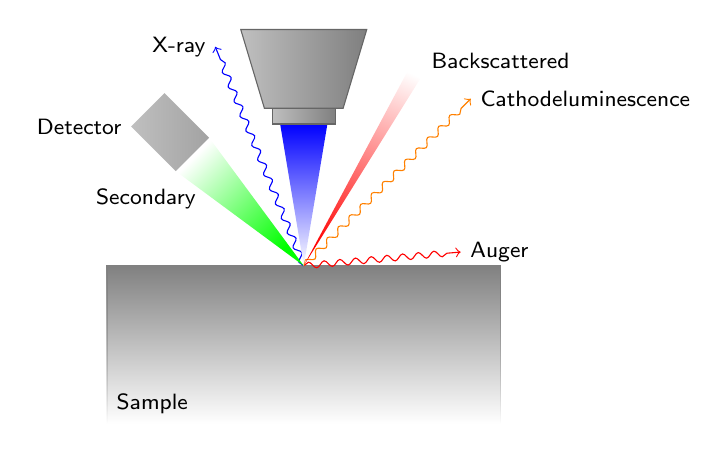
\begin{tikzpicture}
      \draw[gray,fill=gray,path fading=south] (0,0) rectangle +(5,-2);% sample
        \begin{scope}[decoration={snake,amplitude=.4mm,
            segment length=2mm,post length=1mm}]
          \draw[decorate,blue,->] (2.5,0) -- ++(112:3);% x-ray
          \draw[decorate,red,->] (2.5,0) -- ++(5:2);% auger
          \draw[decorate,orange,->] (2.5,0) -- ++(45:3);% cathodlimuescence
        \end{scope}
      \fill[color=red, path fading=north,fading transform={rotate=-15}]
        (2.5,0) ++(60:3) ++(150:0.1) -- ++(-30:0.2) -- (2.5,0) -- cycle;%backscatter
      \fill[color=green, path fading=north,fading transform={rotate=45}]
        (2.5,0) ++(135:2) ++(225:0.3) -- ++(45:0.6) -- (2.5,0) -- cycle;%secondary
      \shade[inner color=blue, top color=blue] (2.2,1.8)
        -- ++(0.6,0) -- ++(-0.3,-1.8) -- cycle;%primary electrons
    
      \shade[left color=gray!50!white,right color=gray] (1.7,3)
        -- ++(1.6,0) -- ++(-0.3,-1) -- ++(-1,0) -- cycle;% column
      \shade[left color=gray!50!white,right color=gray] (2.1,2)
        -- ++(0.8,0) -- ++(0,-0.2) -- ++(-0.8,0) -- cycle;% column bottom
      \draw[gray!80!black] (1.7,3) -- ++(1.6,0) -- ++(-0.3,-1)
        -- ++(-1,0) -- cycle;%column
      \draw[gray!80!black] (2.1,2) -- ++(0,-0.2) -- ++(0.8,0)
        -- ++(0,0.2);%column bottom
            
      \shade[left color=gray!50!white,right color=gray] (2.5,0) ++(135:2) --
        ++(225:0.3) -- ++(135:0.8) -- ++(45:0.6) -- ++(315:0.8) -- cycle;% detector
            
      %labels
      \draw (0,-2) node[above right] {\footnotesize Sample};
      \draw (2.5,0) ++(5:2) node[right] {\footnotesize Auger};
      \draw (2.5,0) ++(45:3) node[right] {\footnotesize Cathodeluminescence};
      \draw (2.5,0) ++(60:3) node[right] {\footnotesize Backscattered};
      \draw (2.5,0) ++(112:3) node[left] {\footnotesize X-ray};
      \draw (2.5,0) ++(135:1.2) node[left=0.4cm] {\footnotesize Secondary};
      \draw (2.5,0) ++(135:2) ++(225:0.3) ++(135:0.8) node[left]
        {\footnotesize Detector};
    \end{tikzpicture}
    \end{document}